\documentclass{article}
\usepackage{tikz}
\usetikzlibrary{arrows.meta}

\begin{document}

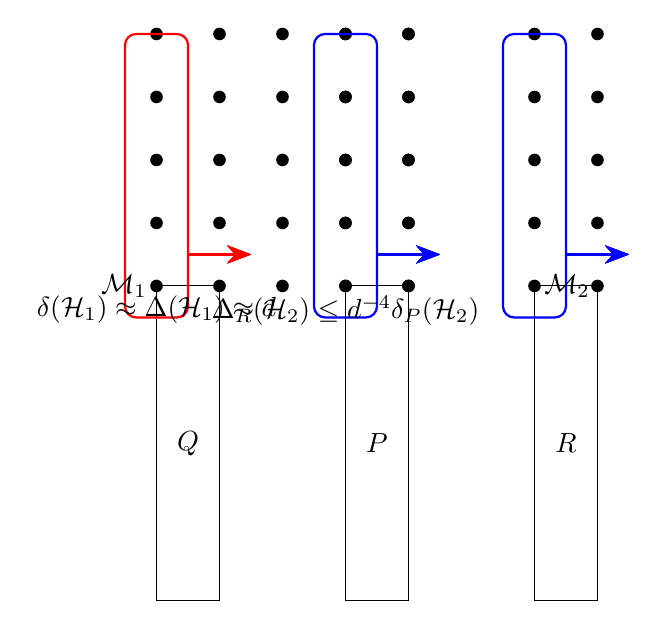
\begin{tikzpicture}[scale=0.8]
    % Define coordinates for nodes
    \coordinate (Q) at (-3,0);
    \coordinate (P) at (0,0);
    \coordinate (R) at (3,0);
    
    % Draw the nodes
    \draw[fill=white] (Q) rectangle ++(1,-5) node[midway] {$Q$};
    \draw[fill=white] (P) rectangle ++(1,-5) node[midway] {$P$};
    \draw[fill=white] (R) rectangle ++(1,-5) node[midway] {$R$};
    
    % Draw the dots inside the nodes
    \foreach \x in {0,...,4} {
        \foreach \y in {0,...,4} {
            \fill (Q) ++(\x,\y) circle (0.1);
        }
    }
    \foreach \x in {0,...,1} {
        \foreach \y in {0,...,4} {
            \fill (P) ++(\x,\y) circle (0.1);
        }
    }
    \foreach \x in {0,...,1} {
        \foreach \y in {0,...,4} {
            \fill (R) ++(\x,\y) circle (0.1);
        }
    }
    
    % Draw the matchings
    \draw[red, thick, rounded corners] (Q) ++(-0.5,-0.5) rectangle ++(1,4.5);
    \draw[blue, thick, rounded corners] (P) ++(-0.5,-0.5) rectangle ++(1,4.5);
    \draw[blue, thick, rounded corners] (R) ++(-0.5,-0.5) rectangle ++(1,4.5);
    
    % Draw the edges of the matchings
    \draw[red, thick, -{Stealth[length=3mm]}] (Q) ++(0.5,0.5) -- ++(1,0);
    \draw[red, thick, -{Stealth[length=3mm]}] (Q) ++(0.5,0.5) -- ++(1,0);
    \draw[red, thick, -{Stealth[length=3mm]}] (Q) ++(0.5,0.5) -- ++(1,0);
    \draw[red, thick, -{Stealth[length=3mm]}] (Q) ++(0.5,0.5) -- ++(1,0);
    \draw[red, thick, -{Stealth[length=3mm]}] (Q) ++(0.5,0.5) -- ++(1,0);
    \draw[red, thick, -{Stealth[length=3mm]}] (Q) ++(0.5,0.5) -- ++(1,0);
    \draw[red, thick, -{Stealth[length=3mm]}] (Q) ++(0.5,0.5) -- ++(1,0);
    \draw[red, thick, -{Stealth[length=3mm]}] (Q) ++(0.5,0.5) -- ++(1,0);
    
    \draw[blue, thick, -{Stealth[length=3mm]}] (P) ++(0.5,0.5) -- ++(1,0);
    \draw[blue, thick, -{Stealth[length=3mm]}] (P) ++(0.5,0.5) -- ++(1,0);
    \draw[blue, thick, -{Stealth[length=3mm]}] (P) ++(0.5,0.5) -- ++(1,0);
    \draw[blue, thick, -{Stealth[length=3mm]}] (P) ++(0.5,0.5) -- ++(1,0);
    \draw[blue, thick, -{Stealth[length=3mm]}] (P) ++(0.5,0.5) -- ++(1,0);
    \draw[blue, thick, -{Stealth[length=3mm]}] (P) ++(0.5,0.5) -- ++(1,0);
    \draw[blue, thick, -{Stealth[length=3mm]}] (P) ++(0.5,0.5) -- ++(1,0);
    \draw[blue, thick, -{Stealth[length=3mm]}] (P) ++(0.5,0.5) -- ++(1,0);
    
    \draw[blue, thick, -{Stealth[length=3mm]}] (R) ++(0.5,0.5) -- ++(1,0);
    \draw[blue, thick, -{Stealth[length=3mm]}] (R) ++(0.5,0.5) -- ++(1,0);
    \draw[blue, thick, -{Stealth[length=3mm]}] (R) ++(0.5,0.5) -- ++(1,0);
    \draw[blue, thick, -{Stealth[length=3mm]}] (R) ++(0.5,0.5) -- ++(1,0);
    \draw[blue, thick, -{Stealth[length=3mm]}] (R) ++(0.5,0.5) -- ++(1,0);
    \draw[blue, thick, -{Stealth[length=3mm]}] (R) ++(0.5,0.5) -- ++(1,0);
    \draw[blue, thick, -{Stealth[length=3mm]}] (R) ++(0.5,0.5) -- ++(1,0);
    \draw[blue, thick, -{Stealth[length=3mm]}] (R) ++(0.5,0.5) -- ++(1,0);
    
    % Labels
    \node at (Q) [left] {$\mathcal{M}_1$};
    \node at (R) [right] {$\mathcal{M}_2$};
    \node at (Q) [below] {$\delta(\mathcal{H}_1) \approx \Delta(\mathcal{H}_1) \approx d$};
    \node at (P) [below] {$\Delta_R(\mathcal{H}_2) \leq d^{-4}\delta_P(\mathcal{H}_2)$};
\end{tikzpicture}

\end{document}